\documentclass[a4,landscape]{book}


\usepackage[margin=1in]{geometry}

\usepackage{multirow}

\usepackage{multicol}

\usepackage{microtype}

\usepackage{accanthis}

\usepackage{graphicx}

\usepackage{fancyhdr}

\pagestyle{fancy}
\chead{MSARPG: A Small RPG}


\title{MSARPG}

%\subtitle{A Small RPG and Some Adventure Ideas}

\author{Sam Wallace}


\begin{document}

%\maketitle
\begin{multicols*}{4}
\chapter*{MSARPG}

Sam Wallace

\subsection*{Introduction}
Minimalist setting-agnostic RPG (MSAPRG) is a role--playing game and adventure inspiration pack.
The game rules are setting agnostic, but this document includes several concepts for situations to get you started playing.
The rules are minimalist, in that there are rules that encompass broad categories of situations, but no rules for the specific actions a player might take.
It will be up to the players and the Referee of the game to come to agreement on how rules apply. \\

The situations are simply stated as adventure hooks, without any definite conclusion written in them.
The situation should get you through 3-4 hours of gameplay; beyond that, follow up on what players find interesting and want to do. \\

This game should be played more like a freeform game of improvisation than scripted like a movie; you should have fun by collaboratively storytelling and working together to create a dramatic story. \\

My inspiration for this ruleset comes from the amazing work of Highland Paranormal Society (Tunnel Goons), Jason Tocci (24xx games), and Ben Milton (Maze Rats).

\subsection*{Rules}
Every player gets a character, except the Referee who runs the rest of the world.
Player characters have 3 traits, Strength (STR), Dexterity (DEX), and Acumen (ACU).
Each of these get a bonus associated to them, ranging from +0 to +3 (no higher is allowed).
To determine your bonuses, roll two six-sided dice (2d6), then assign bonuses that total to the lower of the two rolls. 
Player characters also have inventory slots, generate similarly by taking the lower roll of a 2d6 roll. \\

Players may also start with, or gain throughout play, items, powers, or proficiencies as seems fit to their character and the setting. \\

Player characters will encounter dangerous or risky situations throughout play, or need to resolve contested actions.
Players will roll to determine the result.
Only roll if there is a clear and present risk, danger, or constraint that prevents clear success or failure. \\

Make a decision roll by rolling 2d6, totaling the results, and adding any any appropriate bonuses.
If the result is 10 or greater, thing work out in the player characters' favor.
If 10 seems to hard for the task, instead pose an alternative cost (e.g. time, resources).
If 10 seems to easy, make it impossible for the character with their current resources or plan. \\

Examples to roll decisions:

\begin{itemize}
\item Act before someone else in combat (DEX)
\item Endure extreme environmental hazard (STR)
\item Translate an alien language (ACU)
\end{itemize}

Track health and damage with hitpoints.
Each player starts with 2d6 hitpoints and an armor value of 6 (which could be boosted by items.
When damage is rolled for a hit, first subtract from the armor value from the damage, then subtract the result from hit points.
If you drop to 0, you are incapacitated and barely hanging on for life.
If you drop below 0, you die.

To roll damage, roll 2d6 and add STR stat bonus for a melee attack, and DEX stat bonus for a ranged attack.

On ANY 2d6 roll, if doubles are rolled, the consequences of action are modified.
Doubles on a success exceeds the original goal, giving additional benefits and advantages.
Doubles on a failure are catastrophic. 

\subsection*{How to Referee a Game}

Choose a setting whose usual characters, scenarios, and tropes are familiar to you.
Sketch a small map of a starting location.
Write 5-10 bullet points about encounters which would be cool.
Don't label the map.
Create characters and distribute items to them as fits the setting and character; use supplementary material as much as needed. \\

During the game, explain the immediate situation fully.
Let players freely ask clarifying questions to gather as much information as possible.
When players ask to do something, describe a logical consequence, and add complications, advancements, or other developments as seems interesting. \\

Prep as little as possible to enable maximum flexibility.
Don't get in the way of players' ideas; let them succeed at plausible actions.
If an action is cool, consequential, or mission-critical, get into as much detail as possible about how it is carried out.
Never let just a roll determine an outcome.
Make obstacles difficult via hard choices and dilemmas, not more rolls. \\

\subsection*{How to Be a Player}

Have a strong character concept.
Be collaborative with the other players and the referees in the goals you want to achieve; play off of each other to create an interesting group.
Take the Referee's information on good faith and play into what they set up for you.
Be clear about your intentions and work with others to achieve any common goals. \\

\subsection*{Other Advice and Design Intent}

\begin{itemize}
\item Rolling should be easy. You should never have to look up a rule.
\item Encourage in--world advancement and consequences (as opposed to mechanical).
\item Use dice--rolling to abstract important actions as little as possible.
\end{itemize}

\section*{Adventure Hooks}

These adventure hooks are to get you started on a session.
You may continue as your group enjoys, or simply stop when the story runs out.
Continue the adventure in a direction that seems interesting to the group members. \\

All of these hooks are formatted the same way.
``What if we were [group] doing [mission] in [setting], but [obstacle]?''
This format

\begin{itemize}
\item presents a clear group identity for which specific characters can be created around
\item gives a clear goal for the group, which sets the course of the session
\item sets the setting, giving a clear idea of what kind of tropes are to be presented
\item sets up an obstacle, which creates a dramatic tension between the mission success and character capabilities
\end{itemize}

I present some examples of hooks here.\footnote{All of the art in the adventure hooks is public domain.}
Feel free to use them only as inspiration, taking little if nothing else.
They also give an indication of setting via tables of suggested items and possible encounters.

\subsection*{What If...}

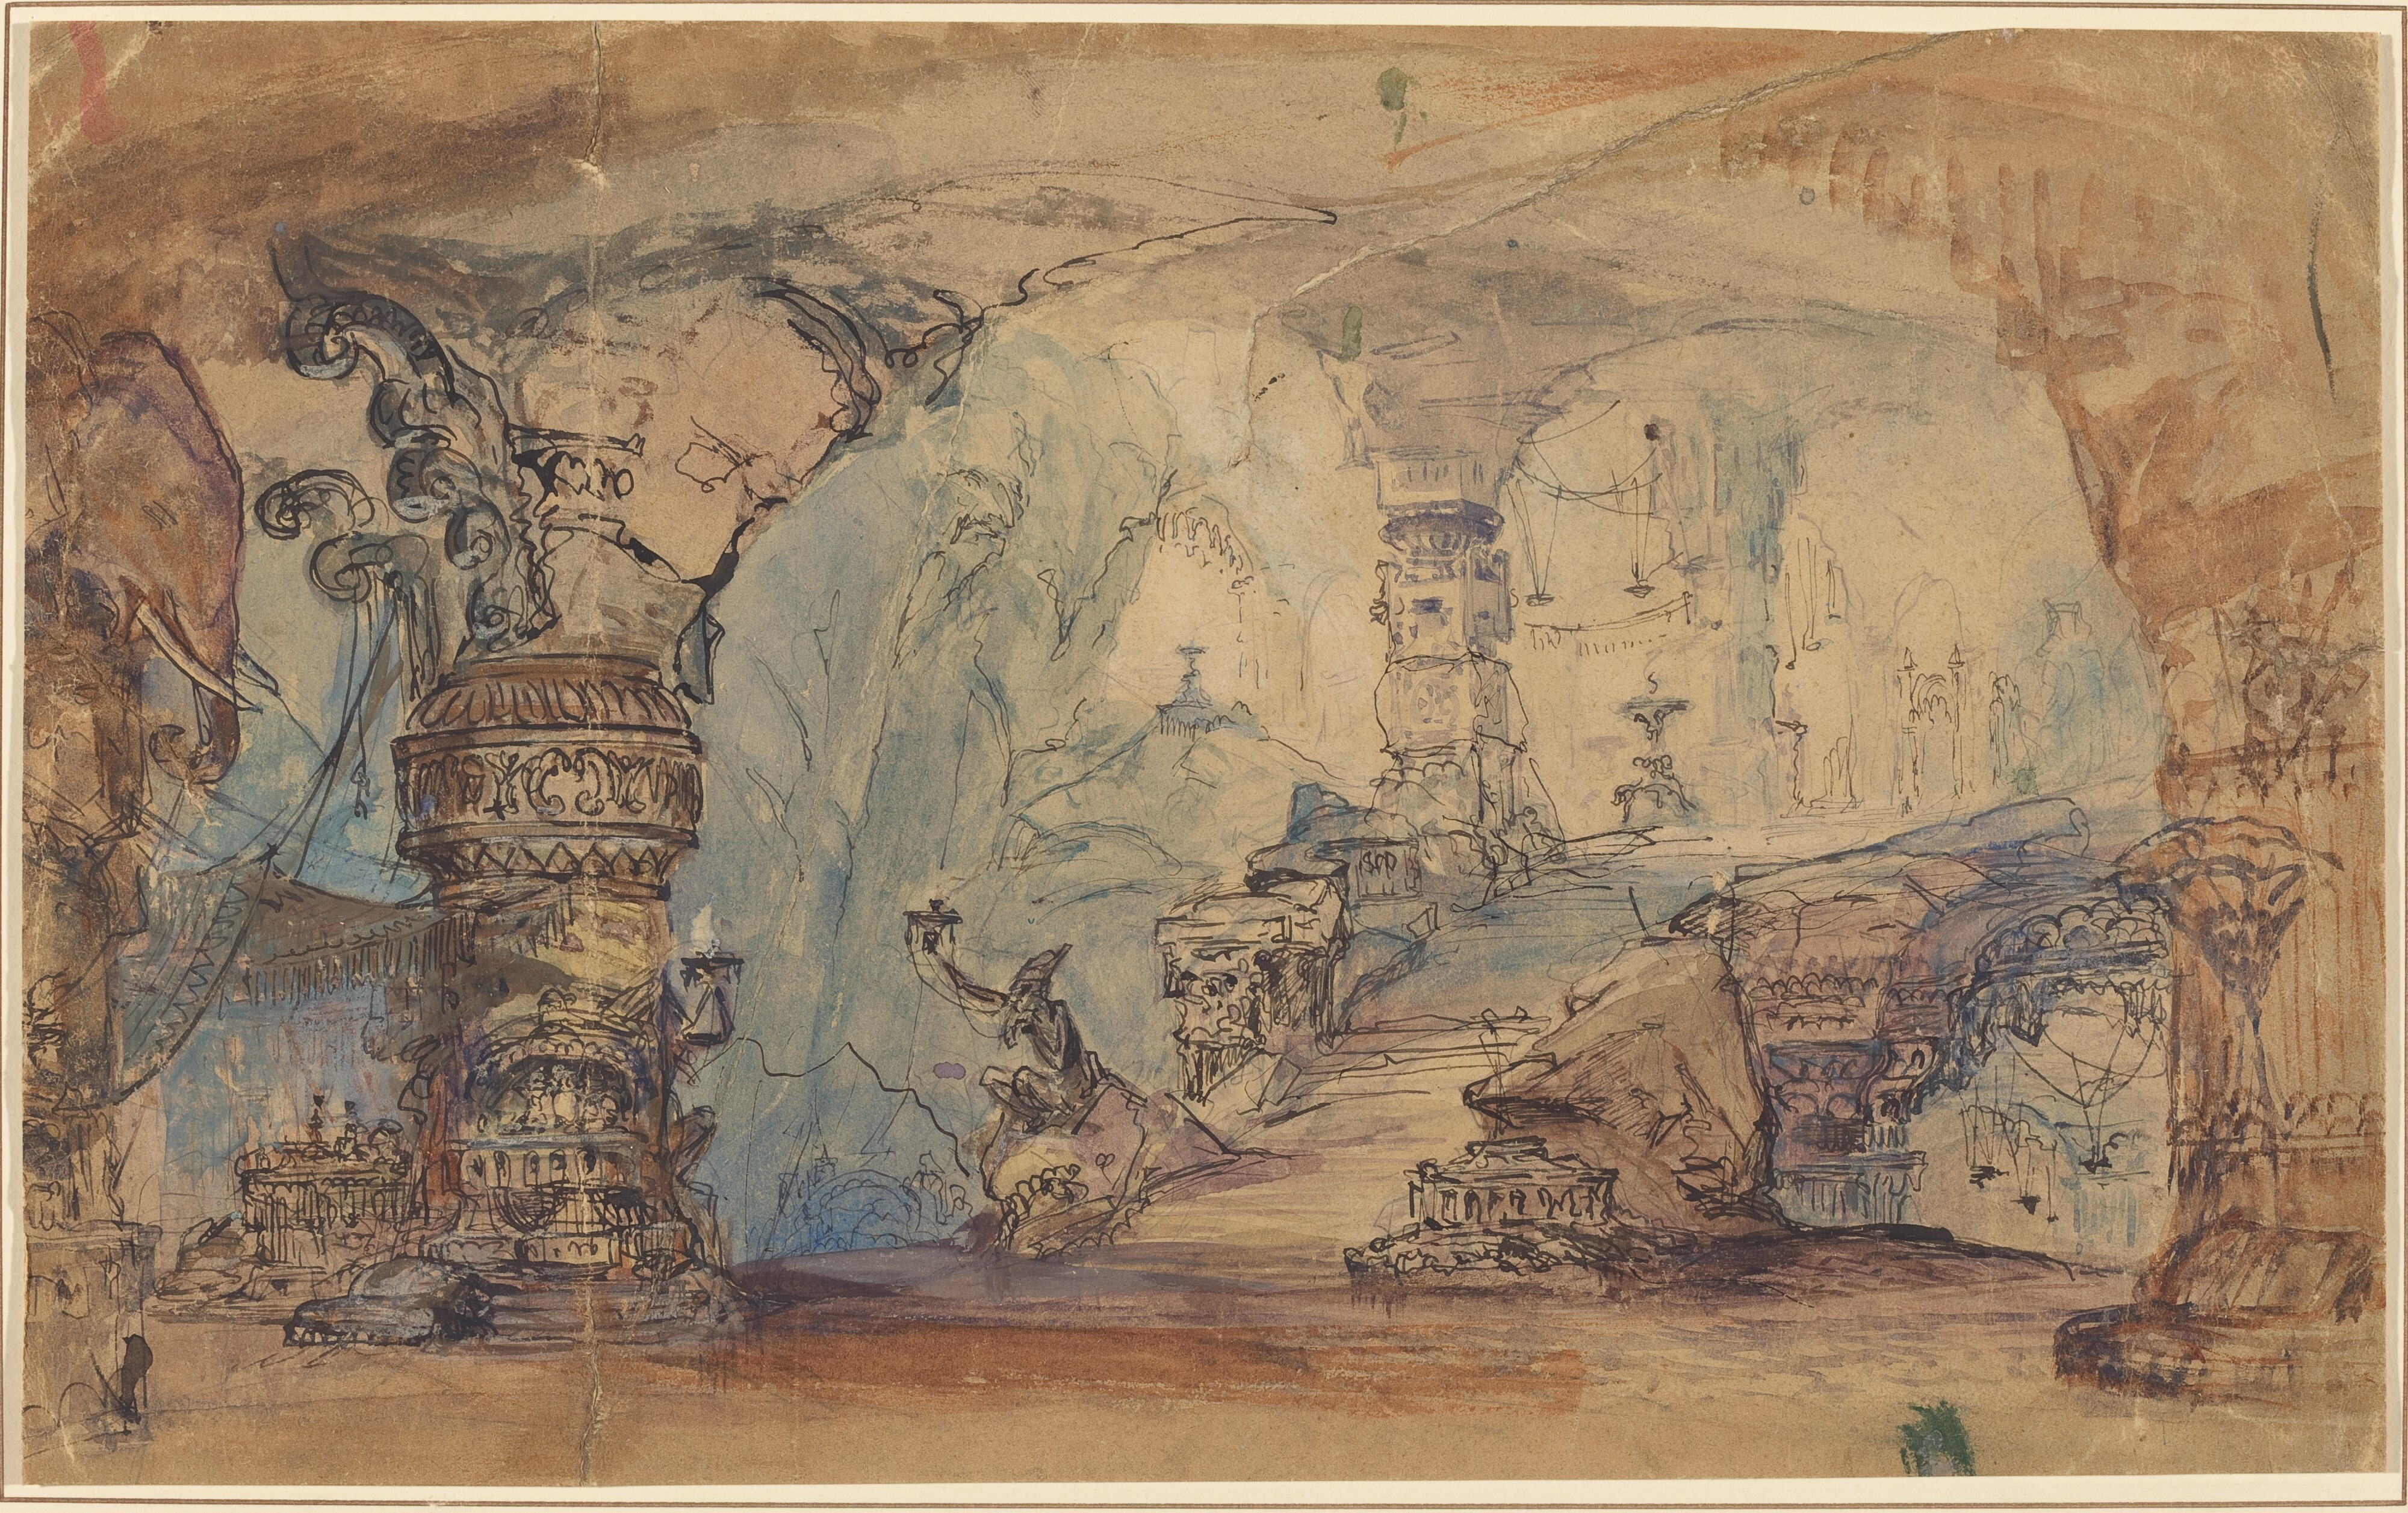
\includegraphics[width=\columnwidth]{./fantastic_cave}

We were forensic engineers investigating a mine collapse deep underground, but the isolation may drive us crazy?
Is there something down there, or is it just our imaginations?
How long can we stay down there and how deep can we go before the paranoia destroys the group? \\

\begin{center}
  \begin{tabular}{|c|l|}
    \hline \multicolumn{2}{|c|}{Items for Forensic Engineers:} \\
    \hline 1 & Air Quality Sensor \\
    2 & Geological Sampling kit \\
    3 & Climbing gear \\
    4 & Subterranean Field Guide \\
    5 & Emergency Flare \\
    6 & Hard Hat \& Headlamp \\
    7 & First Aid Kit \\
    8 & Low Frequency Radio \\
    9 & Mineral Handpick \\
    10 & Respirator \\
    11 & Rubbber Gloves \\
    12 & Sleeping bag \& Tent \\ \hline
  \end{tabular}
\end{center}
\vfill
\columnbreak
\begin{center}
  \begin{tabular}{|c|p{0.8\columnwidth}|}
    \hline \multicolumn{2}{|c|}{Deep Cavern Weirdness:} \\
    \hline 1 & A clatter of rocks off in the distance                                            \\
    2 & Subterranean pool with blind fish                                                        \\
    3 & A cave of bioluminescent fungus, releasing spores periodically                           \\
    4 & A mineral vein that drastically changes color depending on the angle it is viewed from   \\
    5 & Centipedes the size of an anaconda                                                       \\
    6 & Giant cartilaginous lizards                                                              \\
    7 & Rhythmic knocking on cave walls                                                          \\
    8 & A tree in a field of grass, glowing faintly                                              \\
    9 & A bridge over a chasm where a slight whistling of wind is audible                        \\
    10 & Extremely pale humanoids who don't know there is an above ground world                  \\
    11 & A pit full of skeletons that aren't quite human.                                        \\
    12 & An exit into a dense jungle                                                             \\ \hline
  \end{tabular}
\end{center}

How do players get drawn deeper and deeper into the underground world?
What is the layout of the cave, vast and sprawling or dense and claustrophobic?
What really caused the mine collapse?

\subsection*{What If...}

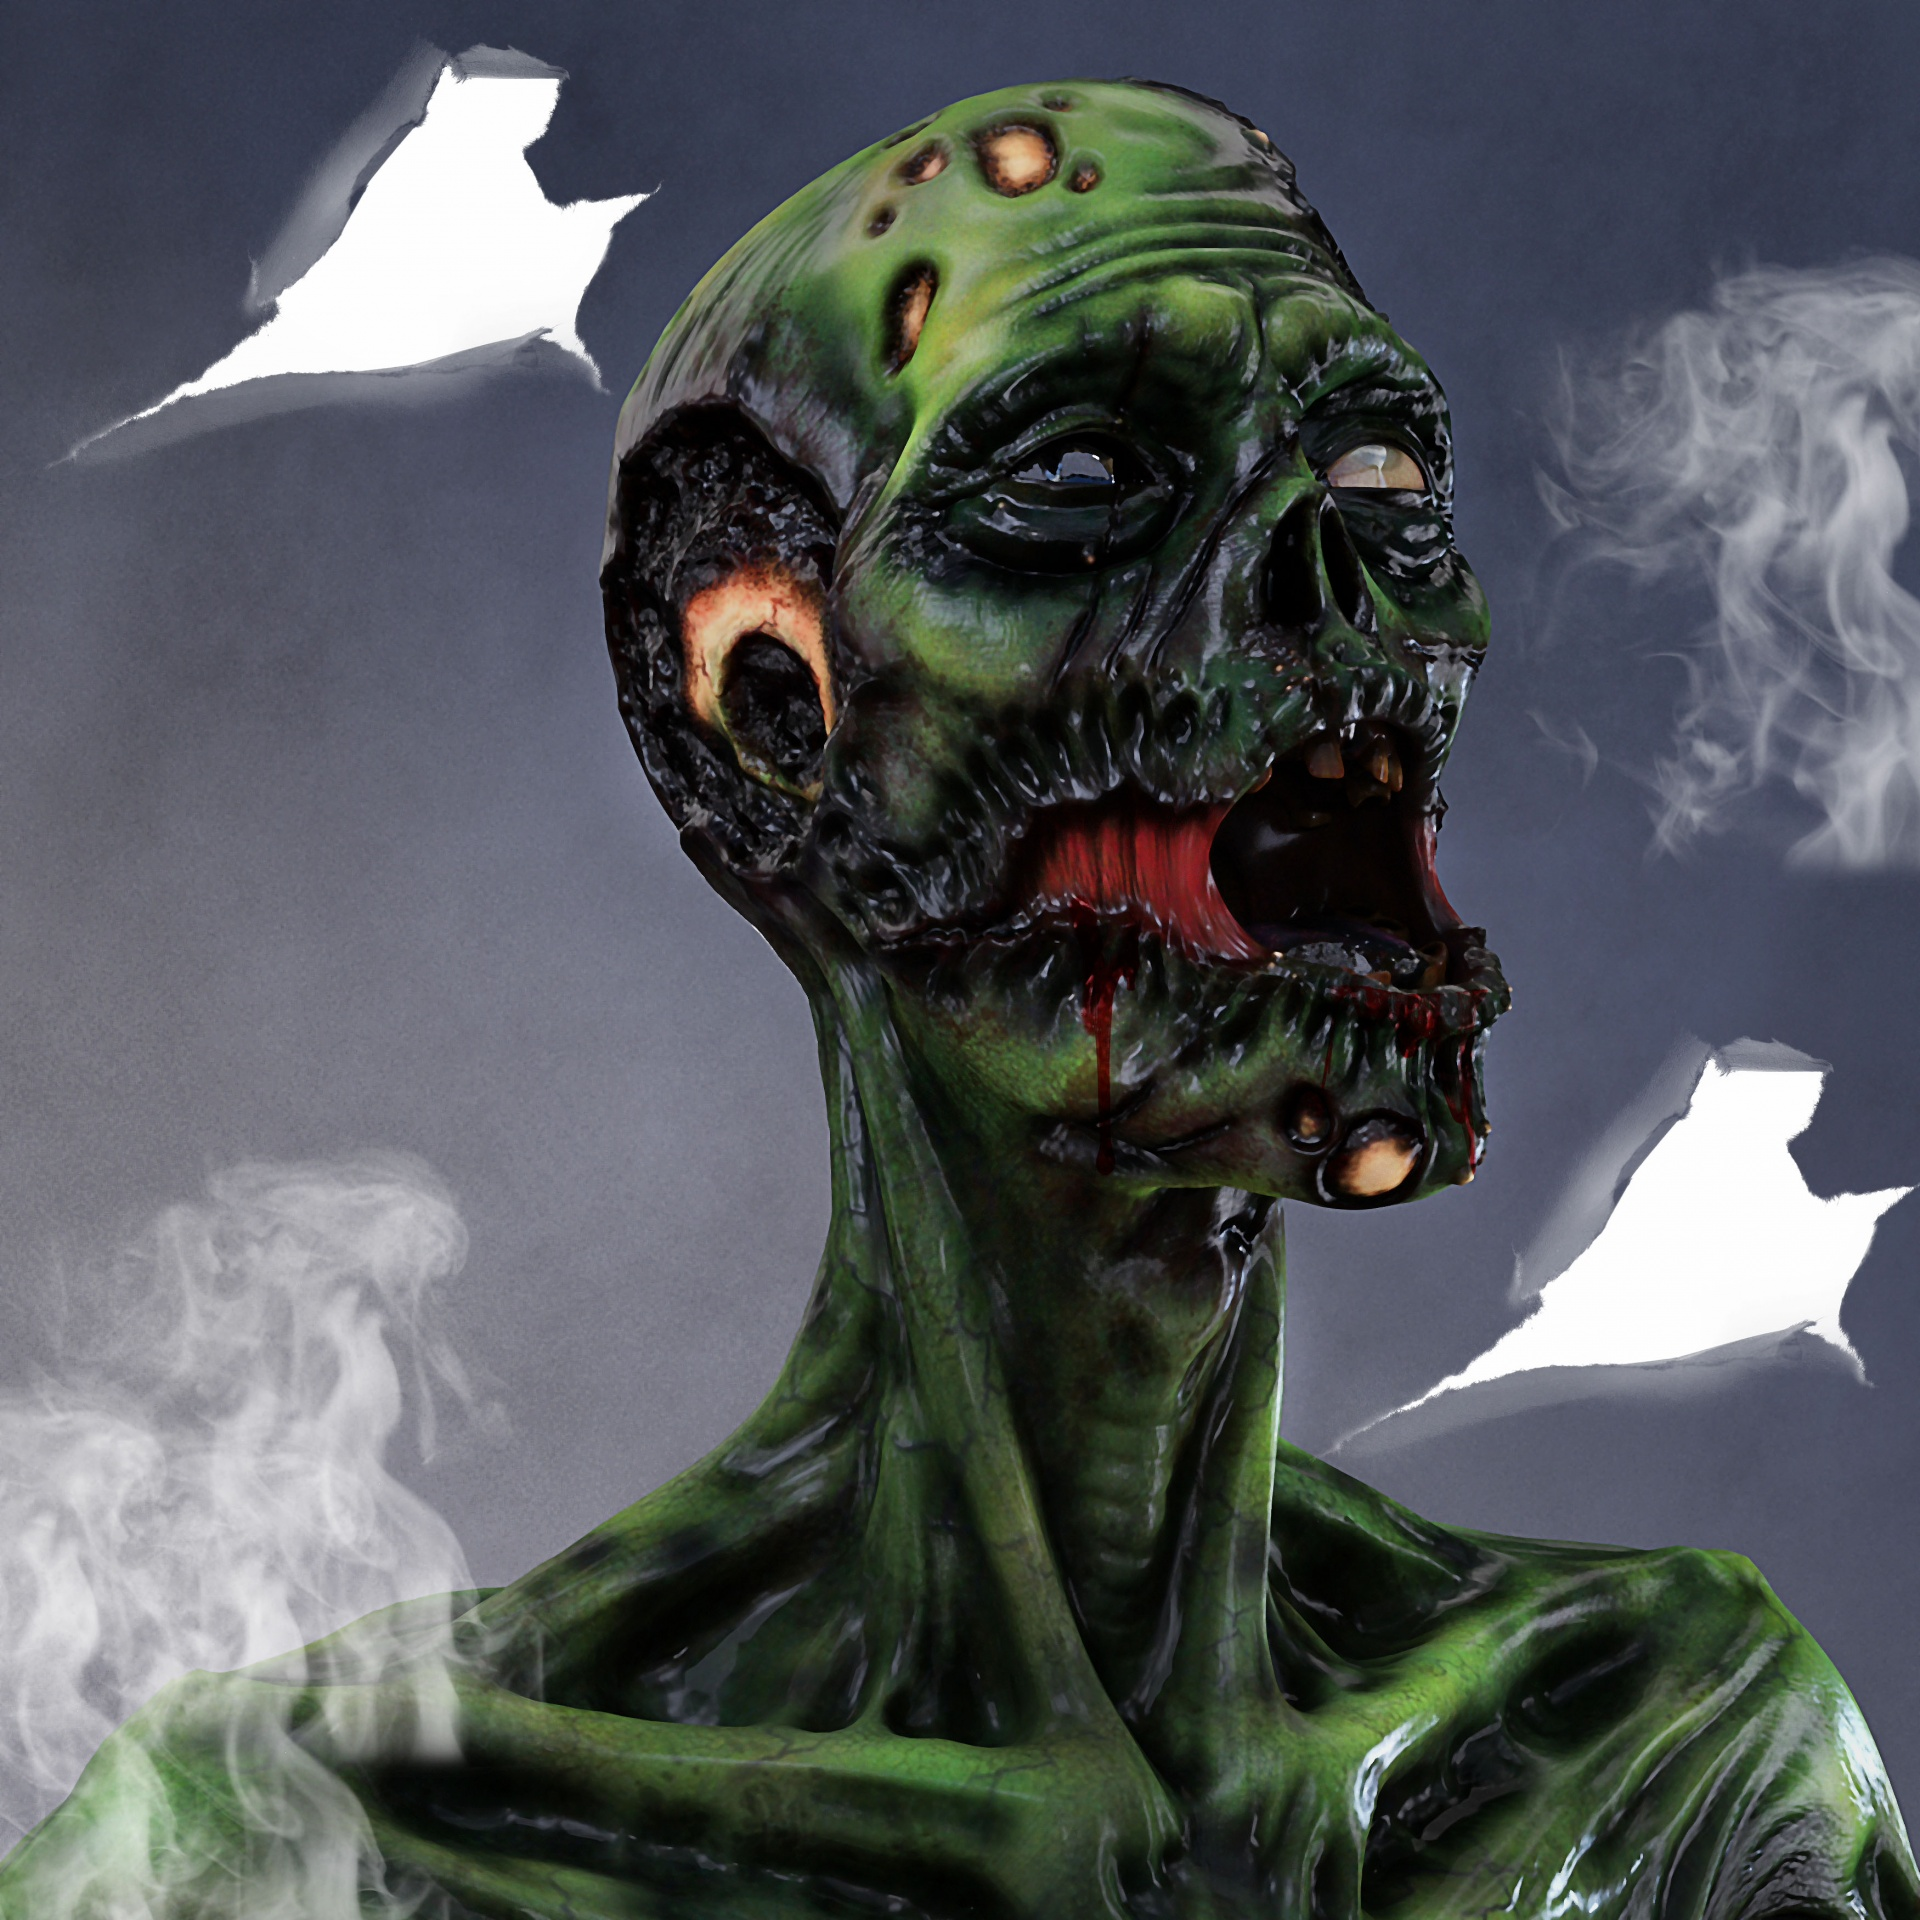
\includegraphics[width=\columnwidth]{./zombie}

We were survivors trying to make it to a safe haven in post--apocalyptic America, but zombies with parasitic fungus crowd the cities?
We've got a van, but do we risk populated areas to get gas for it?
Do we trust that the place we are heading to is truly safe? \\

% What is the population level and density in America now?
% What do people say about the cause of society started?
% What threats other than the zombies present themselves as the survivors travel?

\begin{center}
  \begin{tabular}[ht]{|c|l|}
    \hline \multicolumn{2}{|c|}{Items for Survivors:} \\
    \hline 1 & Sawed--off Shotgun \\
    2 & Bowie Knife \\
    3 & Binoculars \\
    4 & Flashbang \\
    5 & Zip Ties \\
    6 & Crowbar \\
    7 & Bear Trap \\
    8 & Megaphone \\
    9 & Road Flare \\
    10 & Bolt Cutters \\
    11 & Car Pop-a-lock Kit \\
    12 & First-Aid Kit \\ \hline
  \end{tabular}
\end{center}

\columnbreak
\begin{center}
  \begin{tabular}{|c|p{0.8\columnwidth}|}
    \hline \multicolumn{2}{|c|}{Threats to Survivors:} \\
    \hline 1 & A group in a jeep tailing the player characters. \\
    2 & The local military base has set up a temporary camp in a large city. \\
    3 & State prison, descended into anarchy, with its prisoners trapped but free to roam inside. \\
    4 & A lone sniper atop a building, shooting at anyone. \\
    5 & A small town sitting in the crook of a river has been flooded, and people cry out for help from rooftops. \\
    6 & An old priest alone in a small church, reciting prayers. \\
    7 & A couple of hunting buddies ambush passerby and demand supplies at gunpoint. \\
    8 & You enter an area of dense fog, where you can catch glimpses of humanoid figures stumbling around. \\
    9 & An empty farm with a bunker locked from the inside.  \\
    10 & An empty government lab, crawling with deformed creatures. \\
    11 & Collapsed interstate bridge somewhere out in the middle of nowhere. \\
    12 & Coralled zombies inside a chainlink--fenced area. \\ \hline
  \end{tabular}
\end{center}

\subsection*{What If...}

We were a space cleanup crew, ransacking a derelict space station, and we heard something loud move near the reactor chamber?
Do we 


\end{multicols*}
\end{document}